%%
%% This is file `example/ch_intro.tex',
%% generated with the docstrip utility.
%%
%% The original source files were:
%%
%% install/buptgraduatethesis.dtx  (with options: `ch-intro')
%% 
%% This file is a part of the example of BUPTGraduateThesis.
%% 

\chapter{绪论}
\section{研究背景及意义}
随着互联网的发展,云数据中心的规模不断扩大,业务流量不断变化,如何为租户提供可编程的云数据中心网络,如何对云数据中心的流量进行有效的控制,提高带宽的利用率,降低成本,成为目前急需解决的问题。

\gls*{SDN}作为一种新兴的可编程网络架构,有动态配置、可编程及快速响应的特点。其核心思想是将网络控制平面与数据转发平面分离,实现控制平面对数据平面的全局集中化控制;同时对外提供开放的可编程接口,为网络提供可编程能力。控制权的迁移使得底层构架能够抽象出来,各种应用和网络服务因此能将网络当作一个逻辑或虚拟实体,不再依赖于底层网络设备\cite{SDN-1},使得网络配置的自动化程度得到极大提高。通过应用SDN,除了网络的设计和操作变得简化,网络设备也得到简化,这些设备无需理解或处理成千上万的协议,只需要接受SDN控制器的指令即可。利用集中控制,网络管理员可以实时改变网络的行为,并且在几小时或几天内就可以部署新的应用和网络服务。

网络虚拟化\cite{Virtual-1}是一种将底层网络中的硬件以及配套的软件资源进行整合,形成统一管理实体的技术,通过虚拟网络资源到物理网络资源的映射,使得多个逻辑虚拟网络共享底层物理网络基础设施,为用户提供差异化服务。网络虚拟化技术是当今网络革新的重要技术之一。从概念上,网络虚拟化与SDN是互相独立的,但随着近几年网络技术的发展与融合,二者之间的联系变得越来越紧密,SDN的技术相关专题常会提及网络虚拟化技术,网络虚拟化问题的研究也时常会运用到SDN的概念,可见基于SDN的网络虚拟化技术已经成为网络技术研究领域的一个专门课题。

OpenStack\cite{Openstack-1}是由Rackspace和美国国家航空航天局(NASA)合作研发的用于搭建Iaas平台的云计算管理软件。旨在为公共及私有云的建设与管理提供软件的开源项目,主要提供计算、存储、网络服务。OpenStack支持几乎所有类型的云环境,项目目标是提供实施简单、可大规模扩展、丰富、标准统一的云计算管理平台。OpenStack通过各种互补的服务提供了\gls*{IaaS}的解决方案,每个服务提供API以进行集成\cite{Openstack-2}。

在现有OpenStack云平台中,租户网络的创建与隔离仅限于服务器内部,OpenStack无法进行物理服务器之间数据中心网络的管控,跨服务器的通信通过隧道技术实现,该模式无法满足用户多样性的需求,同时无法实现云数据中心带宽资源的有效利用,时常会出现有些链路阻塞严重,而有些链路则处于空闲状态。

本文以此作为出发点,提出了一种多租户虚拟网络定制化管理方案,运用虚拟化技术,为租户提供相互隔离的\gls*{vSDN},完成云数据中心物理资源有效利用的同时,SDN网络由租户自有的控制器实现集中管控,租户可以实时监测当前的流量状况并根据流量状况自定义转发路径,实现对网络的灵活管控,在不降低云平台性能的前提下,实现了OpenStack云平台中租户网络的定制化操作,既提高了安全性,又可以根据当下链路的剩余带宽,进行链路的定制化,提高带宽的利用率。对于租户本身而言,真正实现了租户对全局网络的可控性。对于运营商来说,对物理网络的集中控制可以大大较小网络配置的繁琐性,可以对网络故障实现快速的排查,提高可扩展性。

\section{主要研究内容及创新点}
\subsection{研究内容}
本课题为实现基于SDN的云平台多租户虚拟网络定制化方案,将SDN集成到云数据中心,通过虚拟化技术,为租户提供了可编程的vSDN网络,vSDN网络由租户自由的SDN控制器进行集中管控,租户可以根据当前的链路状况,进行定制化流表的下发,真正实现对网络的灵活定制化操作。主要包括以下三个方面的研究内容:

第一、实现虚拟网络的创建:通过虚拟化技术,实现跨物理服务器,数据中心网络的虚拟化,虚拟网络支持SDN模式,由租户自己的SDN控制器实现集中管控,本文选用\gls*{OVX}\cite{OVX-1}实现虚拟网络的创建。对于底层物理设备来说,OVX是一个控制器;对于租户控制器来说,OVX可以看做是OpenFlow交换机的集合,租户控制器看到的只是一张虚拟网络。OVX最大的优势是紧密结合了SDN,可以发挥SDN的控制与转发分离的强大优势,将创建的虚拟网络指定SDN控制器,从而可以运用SDN的优势,实现对租户虚拟网络的管控。该部分主要对OVX进行二次开发,为其封装手动创建虚拟网络的API接口,完成与OpenStack的集成,实现OVX对OpenStack虚拟机的集中管控。

第二、完成虚拟网络的集中控制:针对租户创建的vSDN网络,由租户自己的SDN控制器进行集中管控,本文为用户提供了集成Ryu控\cite{Ryu-1}制器的定制化镜像。本文为该控制器开发了剩余带宽、已用带宽、链路时延的测量以及定制化流表的下发功能。租户可以进行网络的链路带宽、时延,选取一条最优的数据传输链路,下发定制化流表,从而实现数据传输的可控性。提高带宽利用率的同时,数据传输速率得到了很大的改善。

第三、云平台前端可视化操作:本文为实现租户的便捷操作,在OpenStack云平台上开放了可视化界面操作。其一是用来显示物理数据中心网络,并在数据中心网络上进行租户虚拟网络的创建操作,以及数据中心网络链路时延的显示工作。其二用于实现租户虚拟网络的拓扑展示,虚拟网络带宽、时延的展示,以及定制化链路的选取和流表的下发操作。使用户切身感受到操作的便捷性、对网络可控性。

\subsection{创新点}
针对现有云平台数据中心的不足,本文主要实现了SDN与云平台的结合,将SDN的集中控制、网络的虚拟化集成到云平台中,实现了租户网络隔离的同时,租户可以对网络实现自由控制。相应的创新点主要涉及以下几个方面:

\begin{enumerate}
\item 对于云平台运营商来说,物理网络的集中控制,可以有效的减小网络配置的繁琐性,为数据中心规模的伸缩性提供了便利,对网络的状况可以实现实时监控,同时大大加速了网络的故障修复速度,通过控制侧的日志输出,以及错误模拟,实现快速故障排除。
\item 将虚拟化技术集成到云数据中心,为租户提供相互隔离的vSDN网络,该网络由租户自己的控制器实现集中控制。集中控制的实现,可以让租户指定灵活的数据包转发路径,以及灵活的转发策略。对于自身网络的变化也可以实现即时的应对措施。从而对现有的网络资源进行最有效的利用,减少了网络资源的浪费。租户之间的隔离性,保证了租户数据传输的安全性。
\item 基于包对技术,完成了虚拟网络的链路带宽测量,实现了细粒度的剩余带宽测量,精确度远远高于以前的模式;基于数据包统计的方法,实现了粗粒度的已用带宽的测量;完成了SDN架构下的时延测量。租户根据带宽、时延实现定制化链路的选取,可以有效的利用剩余带宽,将降低数据传输时延,大大加快了数据中心网络的传输速度。
\end{enumerate}

综上所述,基于SDN的云平台多租户虚拟网络定制化方案,对提高云数据中心的带宽利用率,为租户提供可编程的云网络是非常必要的,有助于实现租户网络的定制化操作,同时为运营商进行云数据中心的维护和配置提供了便利。

\section{研究生期间主要工作}
在攻读硕士研究生期间,本文作者认真学习专业相关课程,积极参与实验室的科研工作。认真学习了网络智能研究中心要求的基本课程并取得了满意的成绩,先后参与了实验室多个科研项目。主要的研究方向为智慧云平台的开发工作,在老师和师兄师姐的指导下,对研究课题进行了深入的探索,通过阅读书籍和学术论文夯实理论基础,并进行系统设计、实现和功能测试。主要科研经历和学术成果如下:

参与了国家重点实验室自主课题仪器设备研制类——面向无线业务的网络智能承载验证环境,开发智慧云平台,为租户提供自主可控的SDN云网络;在国家重点基础研究发展计划(973 计划)课题——智慧服务机理与理论中,负责新一代网络架构的调研和撰写工作。

以第一作者的身份发表了两篇EI检索论文,具体为:通过对多租户虚拟网络定制化机制的研究,发表了学术论文《MVNC: A SDN-based Multi-tenant Virtual Network Customization Mechanism in Cloud Data Center》,在论文中提出了一种MVNC的多租户虚拟网络定制化机制,论文已发表于IEEE。通过对\gls*{PSO}算法及网路虚拟化的研究,撰写了学术论文《A PSO-Based Virtual Network Customization for Multi-tenant Cloud Services》,在论文中,提出了一种基于PSO算法的网络虚拟化方案,实验证明相对于传统的基于最短路径的虚拟化算法,性能得到很大提升。同时,在此基础上,完成了多租户云服务中虚拟网络的定制化。论文已被录用,即将发表于ACM。
\section{论文组织结构}
论文总共包括五章,具体内容组织如下:

第一章主要概述了研究背景、意义以及研究的主要内容,包括SDN、OpenStack的背景介绍,本文的主要研究内容以及基于SDN云平台多租户虚拟网络定制化的意义、创新点。

第二章

第三章

第四章

第五章

\section{本章小结}
本章对课题的研究背景进行了描述,阐述了SDN、OpenStack、网络虚拟化等相关技术,并在此基础上确定了研究内容,对研究生期间的主要工作做了简单的概括,最后对论文的组织结构进行了介绍。

\begin{enumerate}
\item 第二章介绍……
\item ……
\end{enumerate}
\begin{itemize}
\item 第二章介绍……
\item ……
\end{itemize}

\definecolor{bg}{rgb}{0.95,0.95,0.95}
\begin{center}
%xleftmargin=0.4\textwidth
\begin{minted}[linenos=false,fontsize=\scriptsize,
				frame=single,framesep=10pt]{python} 
def create():
    pass
class Test():
    def __init__():
        pass
\end{minted}  
\end{center}

图\ref{fig:env1}
\begin{figure}[!htb]
  \centering
  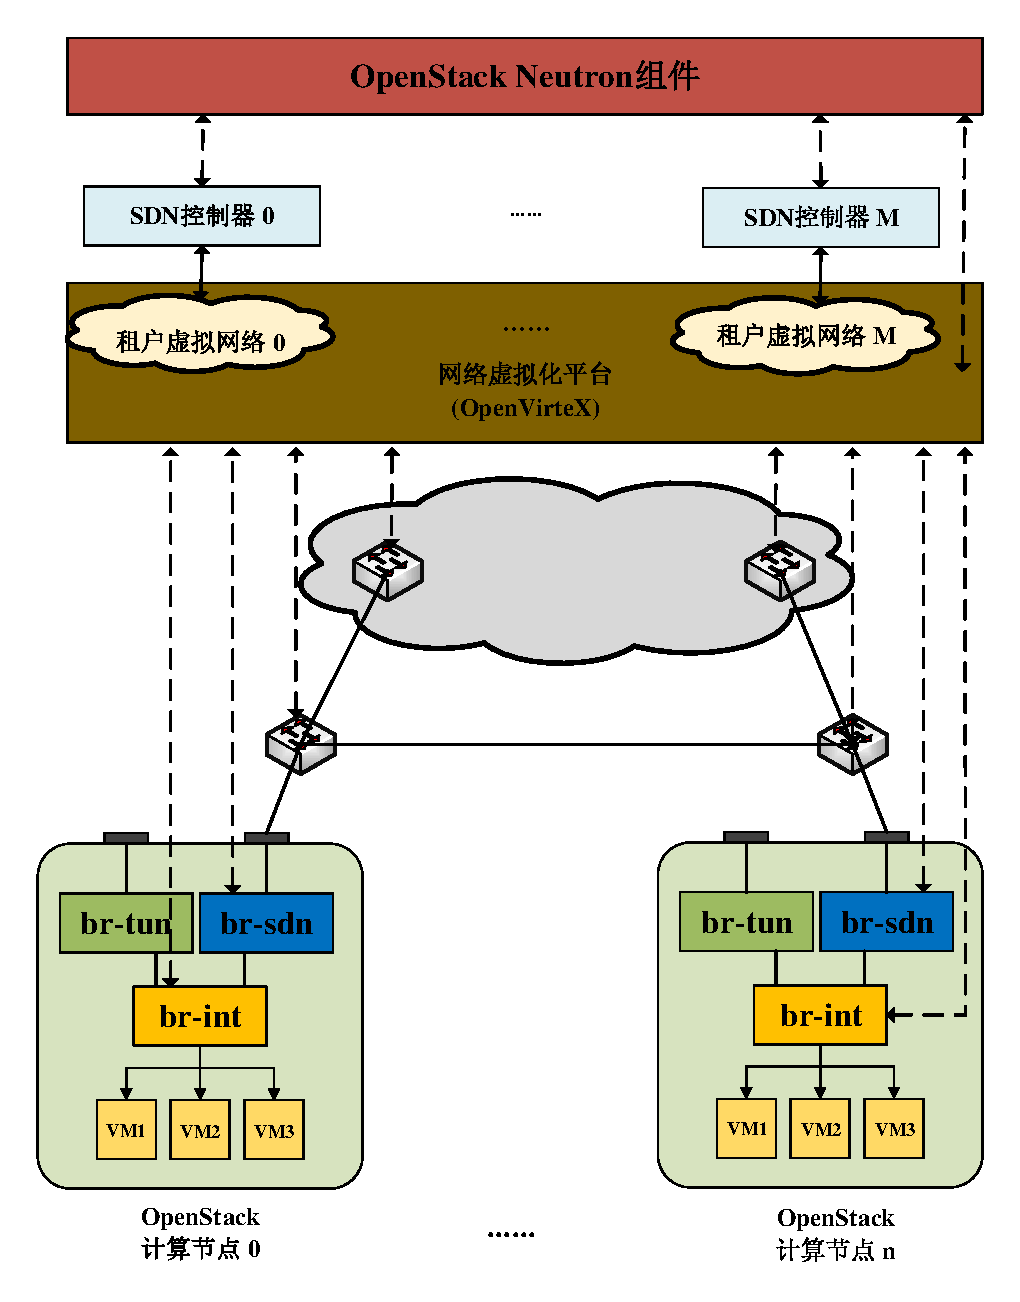
\includegraphics[width=0.6\textwidth]{logo/architecture}
  \caption{System environment.}
  \label{fig:env1}
\end{figure}

脚注使用带圈数字的表示方法,此处为示例 1\footnote{测试脚注一} 和示例 2\footnote{测试脚注二}。
参考文献可以使用\cite{BUPT_Thesis_Format_2014}和\onlinecite{BUPT_Thesis_Format_2004}的表示方法。

%% 本章参考文献
\ifx\usechapbib\empty
\nocite{BSTcontrol}
\setcounter{NAT@ctr}{0}
\bibliographystyle{buptgraduatethesis}
\bibliography{bare_thesis}
\fi
